\documentclass[a4paper, 11pt]{article}
\usepackage{comment} % enables the use of multi-line comments (\ifx \fi) 
\usepackage{fullpage} % changes the margin

\usepackage{mathpazo}

\usepackage[brazil]{babel}                                 
\usepackage[T1]{fontenc} 
\usepackage[utf8]{inputenc}

%legenda ao lado das figuras
\usepackage{sidecap}

\usepackage{subfigure}
\usepackage[pdftex]{graphicx}

\usepackage{hyperref}% add hypertext capabilities

%para nao ficar o retangulo em volta dos links, apenas muda a cor dos caracteres
\hypersetup{ colorlinks,
linkcolor=blue,
filecolor=blue,
urlcolor=blue,
citecolor=blue }

% altera a fonte nas legendas das figuras
\usepackage[font=small,format=plain,labelfont=bf,up,textfont=it,up]{caption}

%%necessario para alguns simbolos matematicos, como \quad
\usepackage{amsmath,amsthm,amssymb}

%packages para usar letras gregas em negrito
\usepackage{bm} %opcao 2
%$\hat{\bm{\varphi}}$

\usepackage[svgnames]{xcolor}
%\usepackage{color} %permite definir cores

%para criar a linha cyan horizontal
\usepackage{stackengine}
\colorlet{lightcyan}{cyan!40!white}


\begin{document}
%Header-Make sure you update this information!!!!
\noindent
\large\textbf{Prova 4} \hfill \textbf{Prof. Paulo Freitas Gomes} \\
\normalsize Física 1 \hfill Curso de Física \\
UFG - Jataí \hfill 23/02/2018 %\\
%TA: Adam Sumner \hfill Due Date: XX/XX/XX




\section*{Problema 1}
Albert Einstein publicou sua Teoria da Relatividade Geral (TRG) em 1916. Várias previsões teóricas já foram observadas experimentalmente mas uma delas só começou a ser testada em 2004, e usa justamente um giroscópio. Na TRG a Terra cria uma distorção no espaço-tempo devido a sua massa. Porém, mais impressionante ainda é que há outra distorção no espaço-tempo criada exclusivamente pela rotação da Terra, como ilustrado na figura \ref{aps_timespace}. Assim, segundo a TRG, um giroscópio em órbita na Terra terá uma precessão devido a essa distorção. Como esperado, esses efeitos não intuitivos e inexistentes em nosso cotidiano são muito pequenos para serem observados. Não obstante, a NASA fez um experimento para tentar detectar essa precessão (uma brincadeira que custou mais de 700 milhões de dólares) \cite{Everitt}. A ideia foi simples: colocar um giroscópio em órbita na Terra e observar se existe uma precessão em seu eixo de rotação devido a rotação da Terra. Foram usados 4 esferas de quartzo brasileiro como giroscópios que ficavam girando com com uma velocidade angular $\omega = 400$ rpm com eixo de rotação apontando para a estrela IM Pegasi (HR 8703). Esta direção serviu como referência e o objetivo era detectar qualquer precessão em relação a essa direção\footnote{Um telescópio acoplado era o responsável por encontrar a estrela guia.}. Um dos efeitos esperados é o deslocamento do eixo de rotação do giroscópio com uma taxa de 40 milisegundos de arco\footnote{Um ângulo de um grau tem 60 minutos de arco e um minuto tem 60 segundos de arco.} por ano. Para manter os eixos de rotação das esferas imóveis, foram produzidas as esferas mais próximas da perfeição da época (2004): diâmetro de 3.8 cm de diâmetro com precisão de 10 $\mu$m (se a Terra fosse uma esfera com a mesma precisão, a maior montanha teria uma altura de apenas 3 metros!). Para efetivamente medir o eixo de rotação, as esferas foram cobertas com nióbio que se torna supercondutor abaixo de 4 K de temperatura\footnote{Para manter essa temperatura durante os 16 meses da missão foram usados 2 mil e 441 litros de hélio líquido.}. Assim, o momento magnético criado (paralelo com o vetor velocidade angular) pode ser medido facilmente usando um SQUID (medidor de magnetização ultrasensível).

\begin{itemize}
\item a) Suponha que o deslocamento observado seja devido a um torque. Calcule esse torque. Dados: densidade do quartzo é 2650 kg/m$^3$.
\item b) Com essa taxa de deslocamento, quanto tempo é necessário para que o eixo de rotação da esfera faça uma volta completa? Para comparação, a precessão da Terra tem período de 26 mil anos.
\item c) Reflitamos um pouco sobre esse efeito: \textit{precessão do eixo de rotação da esfera de quartzo em órbita devido a distorção no espaço tempo criada pela rotação da Terra}. O que isso significa para você?
\item d) Qual o objetivo da física?
\end{itemize}

\begin{figure}
\centering
\subfigure{a)
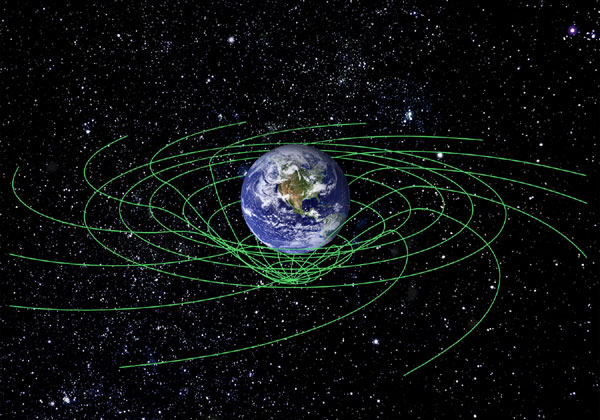
\includegraphics[width=2.8 in]{figuras/aps_timespace.jpg}
\label{aps_timespace}
}
\subfigure{b)
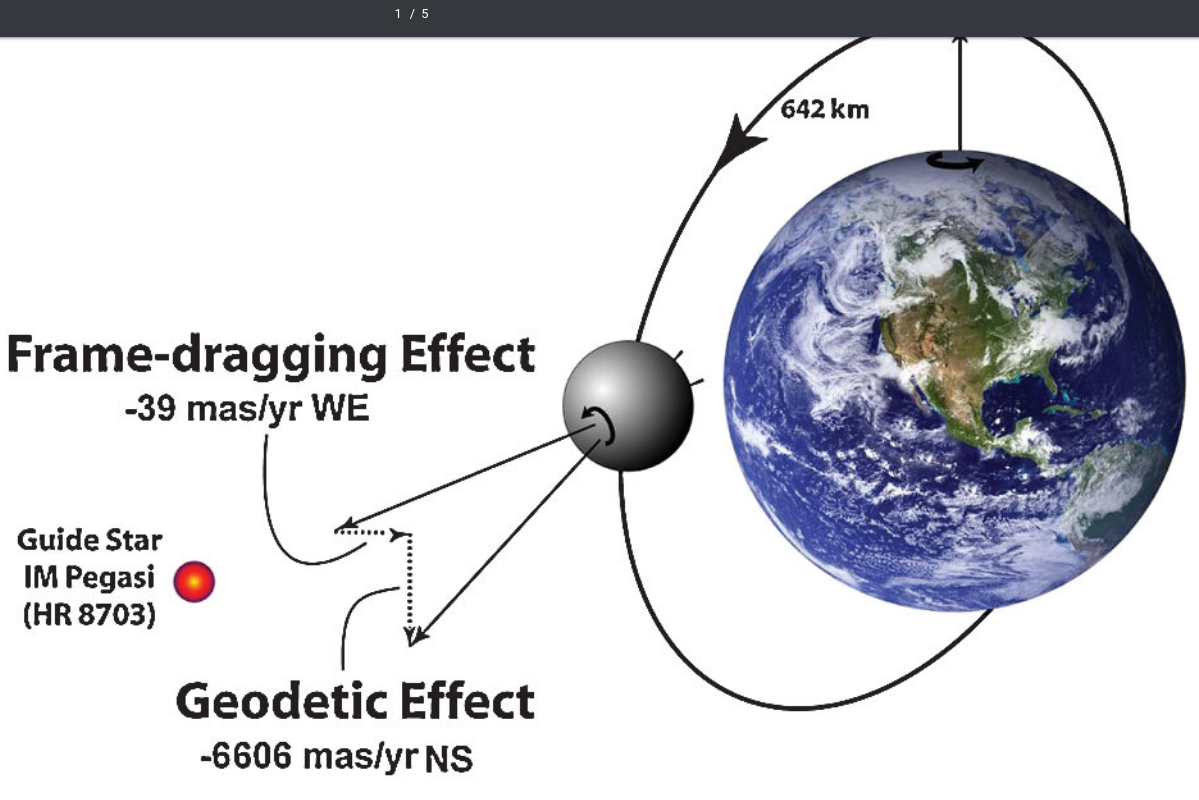
\includegraphics[width=2.9 in]{figuras/gravity_probe_b.png}
\label{gravity_probe_b_2} 
} 
\caption{\subref{aps_timespace} Distorção no espaço tempo provocado pela rotação da Terra. Fonte: \cite{site}. \subref{gravity_probe_b_2} Deslocamentos previstos para o giroscópio de acordo com a TRG. Fonte: \cite{Everitt}.}
\end{figure}


\section*{Problema 2}
Em um laboratório de física você realiza a seguinte experiência de pêndulo balístico: usando uma espingarda de mola você dispara uma bala com massa $m$ e velocidade $v$ na direção da horizontal. A bala fica imediatamente presa a uma distância $r$ abaixo de um eixo sem atrito por um dispositivo de massa $M$ que a retém e que pode girar sem atrito em torno do pivô. O momento de inéria desse dispositivo em torno do pivô é igual a $I$. A distância $r$ é muito maior do que o raio da bala. a) Use a Lei da conservação do momento angular para mostrar que a velocidade agular do sistema logo após o momento em que a bala é retida é dada por $\omega = (mvr)/(mr^2 +I)$. 

b) Depois que a bala fica retida, o centro de massa do sistema bala-dispositivo oscila para cima e atinge uma altura máxima $h$. Use a lei da conservação da energia para mostrar que:
\begin{equation}
h=\dfrac{(mr^2+I)\omega^2}{2g(M+m)}. \nonumber
\end{equation} 


\section*{Problema 3}
O mecanismo indicado na figura é usado para elevar um engradado de suprimentos do depósito de um navio. O engradado possui massa total $M_e$. Uma corda é enrolada em um cilindro de madeira que gira em torno de um eixo de metal. O cilindro possui um raio $R_c$ e momento de inércia $I$. O engradado é suspenso pela extremidade livre da corda. Uma extremidade do eixo está pivotada em mancais sem atrito e uma manivela está presa à outra extremidade. Quando a manivela gira, sua extremidade gira em torno de um círculo vertical de raio $R_m$: o cilindro também gira e o engradado sobe. A massa da corda e o momento de inércia do eixo e da manivela podem ser desprezados. Considere que o engradado está sendo erguido com uma aceleração $a_0$ quando uma força $F$ é aplicada tangencialmente à extremidade da manivela. Perguntas:
a) Usando a Lei de Newton (linear) encontre a tensão $T$ que a corda aplica no engradado.
b) Quais os torques atuantes no sistema cilindro $+$ manivela? Comece escrevendo a definição de torque (lembre-se que é um vetor!).
c) Escreva a Lei de Newton angular (envolvendo momento de inércia e aceleração angular) para o sistema cilindro $+$ manivela.
d) Calcule o módulo $F$ da força na manivela em função de: $T$, $I$, $a_0$, $R_c$ e $R_m$.

\begin{figure}
\centering
\subfigure{a)
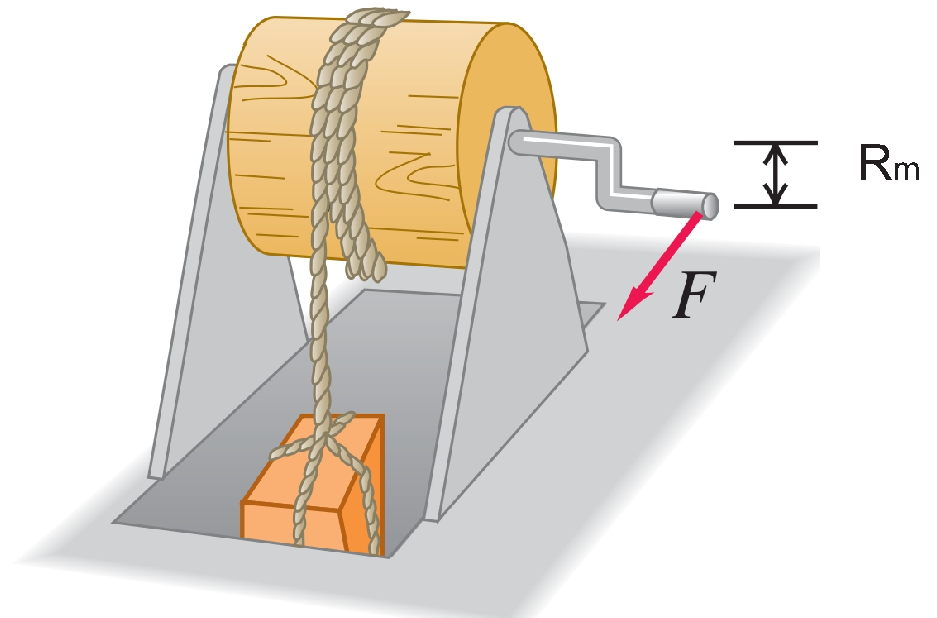
\includegraphics[width=2.8 in]{figuras/guindaste2.pdf}
\label{guindaste2}
}
\subfigure{b)
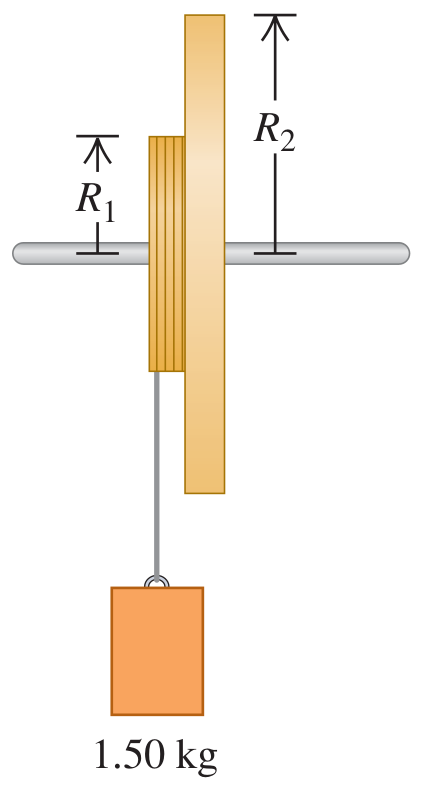
\includegraphics[width=1.5 in]{figuras/discos_R1R2.png}
\label{discos_R1R2} 
} 
\caption{\subref{guindaste2} Ilustração do dispositivo usado no problema 3. \subref{discos_R1R2} Discos referentes ao problema 4. Figuras: fonte \cite{Young2004}.}
\end{figure}

\section*{Problema 4}
Dois discos metálicos, um com raio $R_1=2,5$ cm e massa $M_1 = 0,80$ kg e o outro com raio $R_2= 5,0$ cm e massa $M_2=1,6$ kg, são soldados juntos e montados em um eixo sem atrito passando pelo centro comum (figura). a) Qual é o momento de inércia dos dois discos? b) Um fio fino é enrolado na periferia do disco menor e um bloco de 1,5 kg é suspenso pela extremidade livre do fio. Se o bloco é libertado do repouso a uma distância de 2,0 m acima do solo, qual é sua velocidade no momento em que atinge o solo? c) Repita o cálculo do item (b), desta vez com o fio enrolado na borda do disco maior. Em qual caso a velocidade escalar final do bloco é maior? Explique o por quê.


\section*{Problema 5}
Uma casca esférica de paredes finas com massa $m$ e raio $r$ parte do repouso e rola sem deslizar para baixo da trilha indicada na figura \ref{casca_prob}. O diâmetro da casca é muito pequeno quando comparado com $h_0$ e $R$. O atrito de rolamento é desprezível. a) Calcule a altura mínima $h_0$ necessária para que a casca esférica complete uma volta na parte circular da trajetória? Dica 1: questão 2 da prova 1. Dica 2: pense. b) Suponha que não houvesse atrito e a casca se desloque sem rotacionar. Partindo da mesma algura $h_0$ do item b), mostre que a casca irá completar o loop. Dica: mostre que a velocidade $v_2$ nesse caso no ponto A é maior do que $v_1$ do item b).


\begin{SCfigure}
\centering
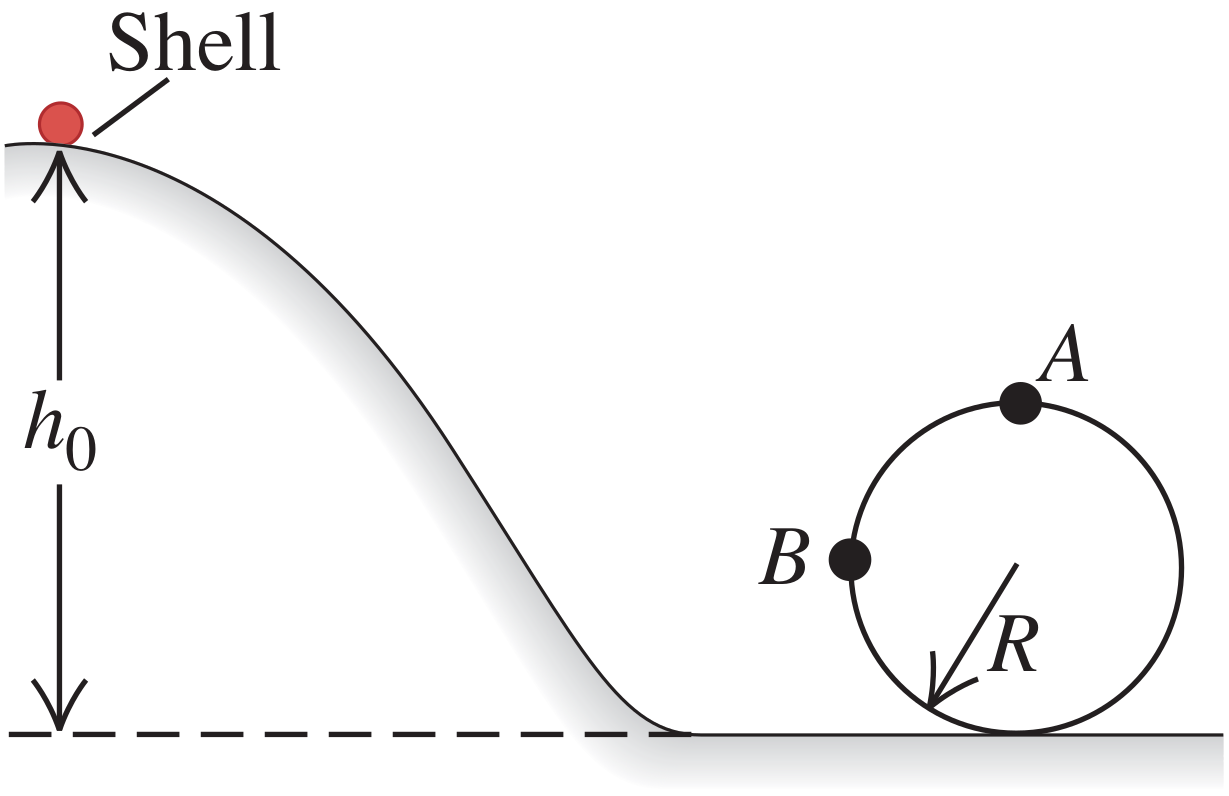
\includegraphics[width=2.5 in]{figuras/casca_prob.png}
\caption{Superfície com a casca esférica (indicada por shell) na posição inicial. Geometria referente ao problema 5. Fonte: \cite{Young2004}.}
\label{casca_prob}
\end{SCfigure}



\begin{figure}
\centering
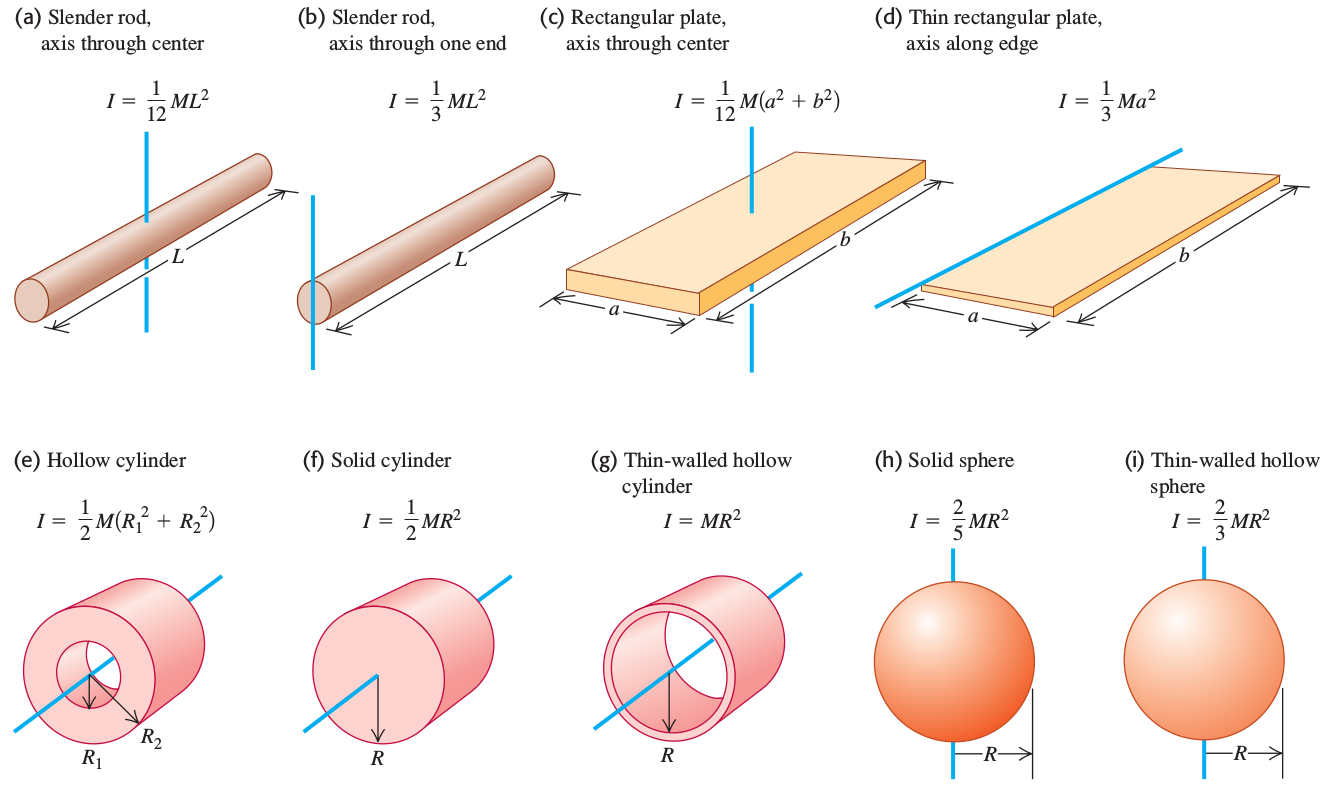
\includegraphics[width=6.0 in]{figuras/tabela_mom_inercia.png}
\caption{Tabela com os momentos de inércia das principais geometrias. Fonte: \cite{Young2004}.}
\label{tabela_mom_inercia}
\end{figure}

{\noindent\def\stackalignment{l}{\textcolor{cyan}{\rule{\linewidth}{2pt}}}\medskip}

\vspace{\fill}

 \begin{flushright}
\begin{small}
\textbf{Uma Receita de Prazer}

O avanço da idade nos faz acordar mais cedo. Deve ser porque dormimos mais cedo, dirão alguns. Não sei. Sempre observei que idosos gostam de madrugar. Meu pai, quando ia viajar, gostava de afirmar: quatro horas da manhã sairemos, é um bom horário, vamos dormir de botas! 
	
Quando cheguei à terceira idade passei a experimentar esta gratificante possibilidade. Sim. Eu gosto de acordar cedo. Aquele silêncio, os primeiros raios de sol, o agradável canto dos pardais, nos levam a uma indizível sensação de paz, a um gosto pela vida, uma alegria pelo retomar de nossas atividades diárias. E eu gosto de rotinas. Então, mãos à obra:

Coloque dois terços de um litro dágua na chaleira, acenda o fogo. Enquanto a água é aquecida, adicione uma colher de açúcar e revolva a água com a colher. Só uma colher de açúcar? Sim, muito açúcar compromente o sabor do café e faz mal à saúde. Se a garrafa térmica já estiver limpa, coloque o coador de papel no suporte, adicione duas colheres de café. Quando a água manifestar o primeiro indício de fervura, derrame sobre o café. Vá completando, na medida em que a água vai se esvaindo do coador, devidamente impregnada de café. Nesse meio tempo sinta o aroma, uma deliciosa mistura de coisas boas, que nos lembram a aurora de nossas vidas. É o recomeço diário de nossa missão na Terra, ser feliz. Por falar em missão, não se esqueça de fechar a garrafa térmica, senão o café esfria. E café frio, dizem, é péssimo! Eu já não gosto de café nem quente, imagine frio. O que? Com toda essa rotina, de monge tibetano, e você não gosta de café? Isso mesmo. Eu gosto de fazer café, não de tomar café. E para quem é esse café cujo preparo é todo roteirizado? Ora, é para alguém que ainda não levantou e que, diariamente, me dá um feedback: hoje seu café está ótimo, um pouquinho forte, mas muito bom. 

Esse “um pouquinho forte” é uma dica para diminuir, uma nesguinha, que seja, na quantidade do pó. Observando as dicas, uma a cada dia, eu fui aperfeiçoando o processo, ajustando os ingredientes, buscando encontrar a satisfação de minha única cliente. Não sou e nem pretendo ser um barista, ainda, mas me defendo bem. E você nunca toma café? O leitor a está a se perguntar. Se eu for a sua casa e você me oferecer um café, eu vou aceitar. Não por que goste de café, mas por que sei reconhecer uma atitude de cortesia.  

\textbf{Antônio Carlos da Costa Gomes.}
\end{small}
\end{flushright}


{\noindent\def\stackalignment{l}{\textcolor{cyan}{\rule{\linewidth}{2pt}}}\medskip}

%%%%%%%%%%%%%%%%%%%%%%%%%%%%%%%%%%%%%%%%%%%%%5
%%%%%%%%%%%Gabarito
%
\newpage
\begin{LARGE}
{\color{red}\textbf{Gabarito}}
\end{LARGE}


\section*{Problema 1}
{\color{red}a) 0,5 ponto.} Supondo que um torque $\tau$ cause a precessão na esfera de quartzo temos que:
\begin{equation}
\Omega = \dfrac{\Delta \theta }{\Delta t} = \dfrac{\tau}{L}, \label{elelkjelkjwre}
\end{equation}
onde $L=I\omega$ é o momento angular da esfera. Seu momento de inércia é $I=(2/5)MR^2$ e o raio é $R = 0,038/2 = 0.19$ m. A densidade de massa é $\rho = M/ V$ onde $V$ é o volume. Para uma esfera $V=(4/3)\pi R^3$, logo a massa é:
\begin{equation}
M = \rho V = \dfrac{4}{3} \rho \pi R^3 =\dfrac{4}{3} \times 2650 \times \pi \times (0,19)^3 \simeq 76,14 \quad \text{kg}. \nonumber
\end{equation}
Já a velocidade angular das esferas é:
\begin{equation}
\omega = \dfrac{4 \times 10^3 \times 2 \pi}{60} = 419 \quad \text{rad/s}. \nonumber
\end{equation}
Para converter segundos de aro em radianos usamos: $\pi$ radianos $= 180$ graus, 1 grau $=$ 60 minutos e 1 minuto $=$ 60 segundos. Logo 1 radiano $= (180/\pi) \times 60 \times 60  = 2,06 \times 10^5 $ segundos. O deslocamento angular é então: 
\begin{equation}
\Delta \theta = \dfrac{ 40 \times 10^{-3} }{2,06 \times 10^5} = 1,94 \times 10^{-7}\quad \text{rad}. \nonumber 
\end{equation}
Esse deslocamento angular ocorre em um ano, logo o tempo é: $\Delta t =365 \times 24 \times 3600 = 3,15 \times 10^7$ segundos. Agora isolamos o torque da Eq. \ref{elelkjelkjwre}:
\begin{eqnarray}
\tau &=& I \omega \dfrac{\Delta \theta}{\Delta t} = (2/5) \times 76,14 \times (0,19)^2 \times 419 \times \dfrac{1,94 \times 10^{-7}}{3,15 \times 10^7}, \nonumber \\
&=& {\color{red}2,84 \times 10^{-12} \quad \text{Nm}}. \nonumber 
\end{eqnarray}

{\color{red}b) 0,5 ponto.}
\begin{equation}
T = \dfrac{2\pi}{\Omega} = \dfrac{2 \pi \Delta t}{\Delta \theta} = \dfrac{2 \pi \times 3,15 \times 10^7 }{1,94 \times 10^{-7}} = {\color{red}1,02 \times 10^{15} \quad \text{segundos} \simeq 32 \quad \text{milhões de anos}}. \nonumber
\end{equation}

{\color{red}c) 0,5 ponto.} A motivação dessa pergunta é o aluno refletir sobre a profundidade teórica do conceito relacionado. Não há uma resposta correta mas é necessário haver uma reflexão concreta e argumentada para ganhar a pontuação correspondente.

{\color{red}d) 0,5 ponto.} A motivação dessa pergunta é o aluno relacionar esse objetivo com o experimento descrito no problema: todo o experimento foi com o intuito de verificar experimentalmente uma previsão teórica da Relatividade Geral, não havia nenhum objetivo aplicado, apenas de confirmar uma teoria física. Uma possível conexão com o texto é que no texto é dito que nossa missão na Terra é ser feliz. A missão da física é o de entender os fenômenos dentro e fora do planeta Terra.

 
 {\noindent\def\stackalignment{l}{\textcolor{lightcyan}{\rule{\linewidth}{2pt}}}\medskip}
 
\section*{Problema 2} 
 
{\color{red}a) 1,0 ponto.} O momento angular é definido como $\textbf{L} = \textbf{r} \times \textbf{p} = m \textbf{r} \times \textbf{v}$ onde $\textbf{r}$ é um vetor que sai de uma origem a ser definida até a posição da partícula. No caso de um movimento retilíneo da bala, escolhemos essa origem no pivô (ponto de rotação) do dispositivo. Logo o módulo é $L = mrv \sin \theta$. No instante imediatamente antes da colisão $\theta = \pi/2$ e assim o momento angular inicial é $L_0 = mrv$ apenas, já que o dispositivo está em repouso. 

Após a colisão a bala fica inscrustrada no dispositivo que oscila com velocidade angular $\omega$. O momento angular agora é $L_1 = I_s \omega$ onde o momento de inércia do sistema é $I_s= mr^2 + I$ e da bala é $mr^2$. Como não há torque externo, a variação do momento angular é nula:
\begin{equation}
\dfrac{d\textbf{L}}{dt} = \bm{\tau} = 0. \nonumber 
\end{equation}  
Logo $L_0= L_1$:
\begin{equation}
mrv = (mr^2 +I) \omega \qquad \qquad \rightarrow \qquad \qquad {\color{red}\omega = \dfrac{mrv}{mr^2 + I}}. \nonumber
\end{equation}

{\color{red}b) 1,0 ponto.} A energia cinética inicial da bala se converte em energia potencial do sistema depois da colisão. Consideremos a altura do centro de massa do dispositivo antes da colisão como sendo $y=0$. Logo a conservação da energia nos dá $K = U$ onde:
\begin{equation}
K = \frac{1}{2}mv^2 = \frac{1}{2} (mr^2 +I) \omega^2, \qquad \qquad U = (M+m)gh. \nonumber
\end{equation}
Logo: 
{\color{red}
\begin{equation}
h=\dfrac{(mr^2+I)\omega^2}{2g(M+m)}. \nonumber
\end{equation}} 

 {\noindent\def\stackalignment{l}{\textcolor{lightcyan}{\rule{\linewidth}{2pt}}}\medskip}

\section*{Problema 3} 

{\color{red}a) 0,5 ponto.}
\begin{equation}
T - M_e g = M_e a_0, \nonumber
\end{equation}
já que o engradado sobre com aceleração $a_0$. Logo: ${\color{red}T = (a_0+g)M_e}$.

{\color{red}b) 0,5 ponto.} A definição de torque é $\bm{\tau} = \textbf{r} \times \textbf{A}$ onde $\textbf{r}$ é o vetor que sai do ponto de referência escolhido e vai até o ponto de aplicação da força $\textbf{A}$. No sistema cilindro $+$ manivela há duas forças atuando: a tensão $T$ da corda puxada pelo engradado e a força $F$ aplicada na manivela. Sendo $\textbf{r}$ perpendicular a $\textbf{A}$ o módulo fica $\tau = rA$. Cada uma gera o seguinte torque em módulo:
{\color{red}
\begin{equation}
\tau_f = R_m F, \qquad \qquad \tau_t = R_c T, \nonumber
\end{equation}} 
já que em ambos os casos a força é perpendicular ao vetor distância.


{\color{red}c) 0,5 ponto.} Tomando o produto vetorial com $\textbf{r}$ em ambos os lados da Lei de Newton temos:
\begin{equation}
\textbf{r} \times  \textbf{F} = \textbf{r} \times  \dfrac{d\textbf{p}}{dt} =  \dfrac{d}{dt}\textbf{r} \times \textbf{p}. \nonumber 
\end{equation}
Logo $\bm{\tau} = d \textbf{L}/dt$. Como a rotação é através do eixo do cilindro $L=I\omega$, a Lei de Newton em módulo fica $\tau = I \dfrac{d\omega}{dt} = I \alpha$, onde $\alpha$ é a aceleração angular.

 O torque resultante é $\tau = \tau_f - \tau_t$ e a aceleração angular é $\alpha = a_0 /R_c$ já que não há deslizamento entre a corda e o cilindro. Usando o resultado do item b) a Lei de Newton angular fica:
{\color{red}\begin{equation}
R_m F - R_c T = I \dfrac{a_0}{R_c}. \nonumber
\end{equation}}

{\color{red}d) 0,5 ponto.} Usando o resultado do item a) no resultado do item c):
\begin{equation}
R_m F - R_c (a_0+g)M_e = I \dfrac{a_0}{R_c} \qquad \Rightarrow \qquad {\color{red}F =  \dfrac{Ia_0}{R_mR_c}+ \dfrac{R_c}{R_m} (a_0+g)M_e}. \nonumber
\end{equation}


 {\noindent\def\stackalignment{l}{\textcolor{lightcyan}{\rule{\linewidth}{2pt}}}\medskip}


\section*{Problema 4} 

{\color{red}a) 1,0 ponto.} 

\begin{eqnarray}
I_s &=& I_1+I_2 = \frac{1}{2}M_1R_1^2 + \frac{1}{2}M_2R_2^2 = \frac{1}{2}0,8 \times (0,025)^2 + \frac{1}{2}1,6 \times (0,05)^2, \nonumber \\
&=&  {\color{red}2,25 \times 10^{-3} \quad \text{kg m$^2$}}. \nonumber
\end{eqnarray}


{\color{red}b) 0,5 ponto.} Vamos aplicar conservação da energia total. Antes, no repouso, há apenas energia potencial gravitacional: $U = mgh$, onde a massa do bloco é $m=1,5$ kg e $h=$ 2 m é a altura inicial. No instante depois há apenas energia cinética do bloco e dos discos: 
\begin{equation}
K = \frac{1}{2}mv^2 + \frac{1}{2} I_s \omega^2. \nonumber
\end{equation}
Como não há deslizamento entre a corda e o disco menor temos que $v_1 = \omega R_1$, logo $\omega = v/R_1$. Da conservação da energia $U = K$:
\begin{equation}
mgh = \frac{1}{2}mv_1^2 + \frac{1}{2} I_s \dfrac{v_1^2}{R_1^2} = \dfrac{m R_1^2 + I_s}{2R_1^2} v_1^2, \qquad \Rightarrow \qquad {\color{red}v_1 = \sqrt{ \dfrac{2mghR_1^2}{m R_1^2 + I_s}  } = 3,4 \quad \text{m/s}} \nonumber 
\end{equation}


{\color{red}c) 0,5 ponto.} Para o disco maior $v_2 = \omega R_2$:
\begin{equation}
{\color{red}v_2 = \sqrt{ \dfrac{2mghR_2^2}{m R_2^2 + I_s}  } = 4,95 \quad \text{m/s}} \nonumber 
\end{equation}
É maior no caso do disco maior pelo seu raio ser maior: a velocidade linear é proporcional ao raio.


 {\noindent\def\stackalignment{l}{\textcolor{lightcyan}{\rule{\linewidth}{2pt}}}\medskip}


\section*{Problema 5} 

{\color{red}a) 1,0 ponto.} Para que a casca esférica complete a volta é necessário que a velocidade mínima no ponto A seja tal que a normal se anule. Aplicando a Lei de Newton $\textbf{F} = m\textbf{a}$ neste ponto:
\begin{equation}
N + mg = m \dfrac{v^2}{R}, \nonumber
\end{equation}
já que a aceleração resultante em um movimento circular é $a_r = v^2/R$. A velocidade será mínima quando $N=0$, o que dá: $v = \sqrt{Rg}$. Agora precisamos calcular o valor de $h_0$ em função dessa velocidade.

Para a conservação de energia definimos o instante antes: há apenas energia potencial gravitacional $U_0 = mgh_0$. Instante depois: energia cinética $K = \frac{1}{2}mv_1^2 + \frac{1}{2} I \omega^2$ e potencial $U_1 = 2mgR$. Como não há deslizamento durante o rolar da casca temos que $I=(2/3)mr^2$ e $v = \omega r$, logo $K = (5/6) mv^2$. Assim:
\begin{equation}
U_0 = K+U_1 \qquad  \Rightarrow \qquad mgh_0 = \dfrac{5}{6} m Rg + 2mgR \qquad \Rightarrow \qquad {\color{red}h_0 = \frac{17}{6}R} \nonumber 
\end{equation}

{\color{red}b) 1,0 ponto.} Neste caso não há energia cinética de rotação $\omega = 0$. Logo $K=\frac{1}{2}mv^2$ de forma que a velocidade da esfera no ponto A será maior do que no caso anterior. Sendo maior, ela conseguirá fazer o loop.

\begin{thebibliography}{99}

\bibitem{Everitt} C. W. F. Everitt \textit{et al} Physical Review Letters \href{ttps://doi.org/10.1103/PhysRevLett.106.221101}{\textbf{106}, 221101 (2011)}.

\bibitem{site} \url{https://news.stanford.edu/news/2007/april18/aps-041807.html}.

\bibitem{Young2004} H. D. Young and R. A. Freedman, \textit{Sears and Zemansky's University Physics with Modern Physics}, 13th Edition, Addison-Wesley (Pearson (2004).


\end{thebibliography}

\end{document}

























